\documentclass {beamer}

\usetheme{Madrid}
\usepackage{url}

\title{Digital Tools for Finance}
\author [Ten, Grigorenko] {Elena Ten \and Elena Grigorenko}
\institute [UZH] {University of Zurich}
\date {15.12.2020}


\AtBeginSection
{
	\begin{frame}
	\frametitle{Overview}
	\tableofcontents[currentsection]

	\end{frame}
}


\begin{document}


\frame{\titlepage}

\section{Overview}
\begin{frame}
\frametitle{Overview}
This set of slides was produced to give an overview of different digital tools, used in our final project.\\
In general, we got experience with Git/Github, Slack, R, Python, SQL, LaTeX (Overleaf and Sublime Text editor) to elaborate the project. 

\end{frame}


% slides

\section{Version Control}
\begin{frame}
\frametitle{Version control}
Version control was implemented via Git. The commands were sent via command line and GitHub desktop.

\end{frame}


\section{Collaboration Tools}
\begin{frame}
\frametitle{Collaboration tools}
We collaborated on the project, using Git.\\
Also we created a Slack channel and connected it to our Git repository.

\end{frame}


\section{Writing with LaTeX}
\begin{frame}
\frametitle{LateX}
We configurated Sublime Text editor to use LaTeX.\\
\begin{itemize}
\item Using Sublime Text and Overleaf, we produced this set of slides as a beamer presentation.
\item Using Sublime Text and Overleaf, we produced the report (report.tex), that contains a table of contents, figures, tables and bibliography.
\item We elaborated the bibliography, having created an auxiliary file \path{/text/biblio.bib}.
\end{itemize}

\end{frame}

\section{Data Management}
\begin{frame}
\frametitle{Data management}
For our project we performed a set of calculations in R (\path{/R/oil_stocks.Rproj}).\\
Specifically we calculated the cost of capital of oil companies with the following steps:
\begin{itemize}
\item Downloaded .csv files with stock and index data
\item Processed and filtered the data in R, using SQL
\item Used regression analysis to estimate historical betas
\item Produced LaTeX output in R
\item Built plots in R
\item Assembled the findings in LaTeX
\end{itemize}

\end{frame}

\section{Visualization}
\begin{frame}
\frametitle{Visualization}

\end{frame}


\section{Knowledge Transfer}
%First slide on Knowledge transfer
\begin{frame}
\frametitle{Knowledge transfer}
With the means of R shiny we produced an interactive page, that processes user's input into graphs (\path{/R/data/app.R}).\\
The application allows user to choose one of the companies and time interval to visualize stock dynamics on a graph. The user may also choose an option to see the dynamics of S\&P 500 on the same graph.\\

% insert screenshot with input
\begin{figure}[!h]
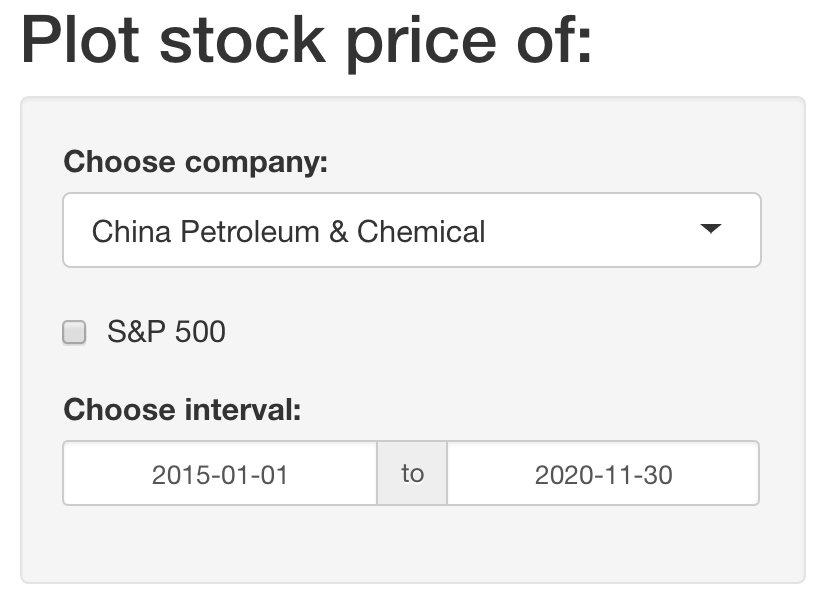
\includegraphics[scale=0.25]{screenshot1}
\label{fig:ss1}
\end{figure}
\end{frame}

%Second slide on Knowledge transfer

\begin{frame}
\frametitle{Knowledge transfer}
Example of output:

% insert screenshot with output2
\begin{figure}[!h]
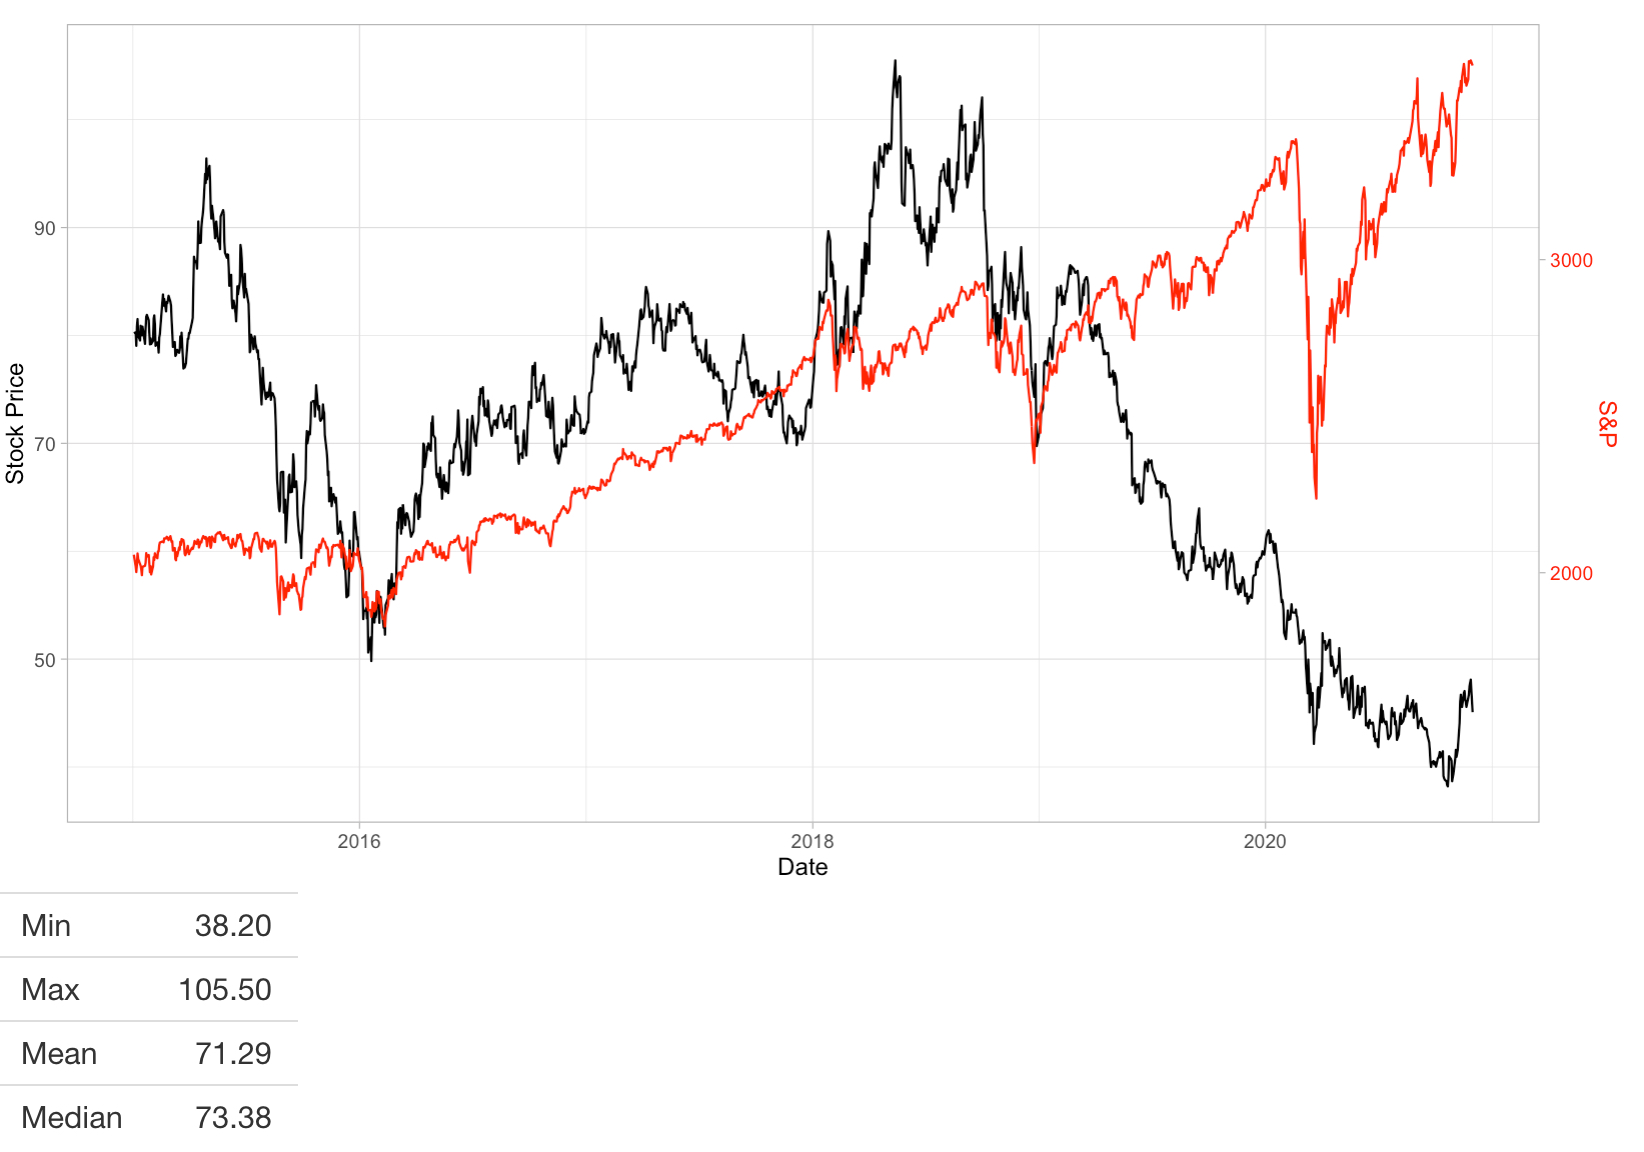
\includegraphics[scale=0.18]{screenshot2}
\label{fig:ss1}
\end{figure}
\end{frame}







\end{document}